\section{Hourly Attenuation Modeling with Stratified Inputs}
\label{sec:hourly_modeling}

This section examines how meteorological input composition and dimensionality affect hourly attenuation estimation. Ten models are first compared along independently constructed feature-elimination paths. A separate TabM experiment then compares vertically resolved and non-vertically-resolved candidate pools at equal retained dimensions. Finally, locally trained models are evaluated at the two UK sites with their parameters and preprocessing fixed.

\subsection{Models, Training, and Evaluation Protocol}
\label{subsec:hourly_protocol}

\subsubsection{Task-adapted TabM}

% P1: Role of TabM and the two candidate input pools in Fig. 5(a).
TabM provides a parameter-efficient ensemble for hourly attenuation estimation by sharing hidden weight matrices across members while retaining member-specific transformations \cite{Gorishniy2025TabM}. Figure~\ref{fig:tabm_architecture}(a) shows its use with the meteorological inputs defined in Section~II. The full candidate pool contains 50 non-vertically-resolved base features and 106 pressure-level features; the base-pool comparison uses the same 50 base features alone. The base features comprise surface quantities, single-level diagnostics, and column-integrated variables. Each pressure-level feature represents one variable at a specified pressure level. At each RFE state, the retained $k$ features describe the observation hour; channel history, timestamps, and weather-category labels are excluded.

% P2: Preprocessing and replication of the same hourly input.
Missing values are filled with medians fitted on the training rows, and each input is standardized using the corresponding training mean and standard deviation. The attenuation target is also standardized for training. For hour $h$, let $\mathbf{x}_h\in\mathbb{R}^{k}$ denote the preprocessed retained input. This vector is replicated across $M=32$ members to form $\mathbf{X}_h\in\mathbb{R}^{M\times k}$, whose rows initially contain the same meteorological information.

% P3: Every matrix and operator in Fig. 5(b); the displayed equation moved here.
Figure~\ref{fig:tabm_architecture}(b) expands one hidden block. Its input $\mathbf{H}\in\mathbb{R}^{M\times d_{\mathrm{in}}}$ is scaled elementwise by the member-specific input adapter $\mathbf{R}$, multiplied by the shared matrix $\mathbf{W}\in\mathbb{R}^{d_{\mathrm{in}}\times d_{\mathrm{out}}}$, and scaled by the member-specific output adapter $\mathbf{S}$. Adding the member-specific bias $\mathbf{B}$, applying ReLU, and applying dropout gives
\begin{equation}
\mathbf{H}'=
\operatorname{Dropout}\!\left(
\operatorname{ReLU}\!\left(
\bigl[(\mathbf{H}\odot\mathbf{R})\mathbf{W}\bigr]\odot\mathbf{S}
+\mathbf{B}
\right)\right),
\label{eq:tabm_hidden_block}
\end{equation}
where $\odot$ denotes elementwise multiplication, $\mathbf{R}$ has the same dimensions as $\mathbf{H}$, and $\mathbf{S}$, $\mathbf{B}$, and $\mathbf{H}'$ have dimensions $M\times d_{\mathrm{out}}$. Rows correspond to ensemble members. Each block has its own $\mathbf{W}$, shared across its members. The network contains three blocks of output width 256, with dropout probability 0.1 during training; dropout is disabled for inference.

% P4: Member-specific heads, training-loss branch and inference-mean branch.
Each member has a separate scalar regression head, denoted by $h_m$ in Fig.~\ref{fig:tabm_architecture}(a), producing a standardized prediction $\widehat{z}_{m,h}$. All members are supervised against the same standardized attenuation target. The training loss is their squared error averaged uniformly over hours and members, as represented by the member-wise MSE branch. For inference, the predictions are averaged to obtain $\overline{z}_h$ and then transformed back to dB:
\begin{equation}
\widehat{A}_h
=\mu_A+\sigma_A\overline{z}_h
=\mu_A+\frac{\sigma_A}{M}\sum_{m=1}^{M}\widehat{z}_{m,h},
\label{eq:tabm_hourly_estimate}
\end{equation}
where $\mu_A$ and $\sigma_A$ are the target mean and standard deviation fitted on the training rows. The shared matrices provide the common nonlinear transformations, while the member-specific scales, biases, and heads distinguish the member predictions without duplicating every hidden weight matrix.

% P5: Training settings and link to the protocol explained in the following text.
The selected network is trained using AdamW with a learning rate of $2\times10^{-3}$, weight decay of 0.01, a batch size of 256, and 54 epochs. Meteorological input construction, training-fitted preprocessing, weather-aware validation, and independent feature-elimination paths adapt the original TabM architecture to this task. The validation criterion and RFE procedure are specified below, and Section~\ref{subsec:uk_frozen_hourly} describes evaluation with the local estimators frozen.

\begin{figure*}[t]
\centering
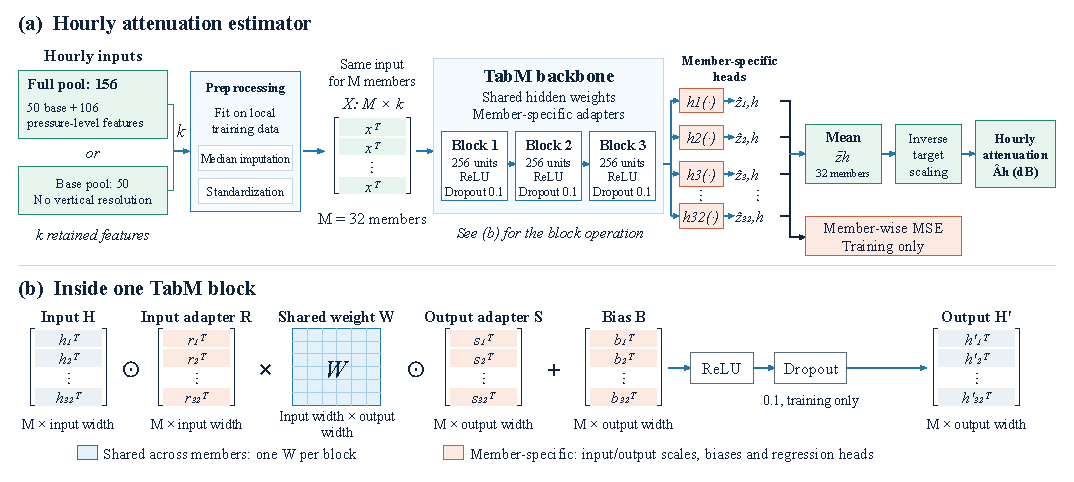
\includegraphics[width=\textwidth]{Fig05_TabM_Architecture_And_Protocol.pdf}
\caption{TabM architecture for hourly attenuation estimation. (a) Preprocessing, parallel member predictions, member-wise training loss, and averaged hourly output. (b) Operations within one hidden block. Blue denotes the hidden weight matrix shared across members; orange denotes member-specific scales, biases, and regression heads. The architecture follows TabM~\cite{Gorishniy2025TabM}. Here, $k$ is the retained input dimension and $M=32$ is the number of ensemble members.}
\label{fig:tabm_architecture}
\end{figure*}

\subsubsection{Comparison models}

Nine comparison models cover several approaches to meteorological regression: a multilayer perceptron (MLP), bidirectional long short-term memory network (BiLSTM), graph convolutional network (GCN), Transformer, Bai LSTM, radial-basis-function support vector regression (SVR-RBF), CatBoost, Random Forest, and Elastic Net.

The MLP uses two hidden layers of widths 64 and 32. BiLSTM, Transformer, and GCN explicitly organize pressure-level variables by vertical position and combine their encoded profiles with a separate base-feature branch. BiLSTM processes the ordered pressure levels in both directions. The Transformer uses two encoder layers with four attention heads and a representation width of 32. GCN uses two graph-convolution layers over neighboring pressure levels, with a gate controlling the contribution of the vertical representation. These three models encode the atmospheric structure within one hour.

The Bai LSTM comparator adapts the LSTM architecture of Bai et al. \cite{Bai2022FeatureSelection} to the same concurrent-meteorology task. It uses one input step, an LSTM hidden width of 32, and fully connected layers of widths 16, 32, 64, and 1. SVR-RBF and Elastic Net provide kernel-based and regularized linear comparisons, while CatBoost and Random Forest provide tree-ensemble comparisons. All ten models use the same candidate measurements and data partitions. Their selected configurations are reported in Table~\ref{tab:Table03_Training_And_RFE_Protocol}.

% Table 3: configurations and common experimental protocol.
% Generated by build_tables.py; source files: Table03_model_configs.json, methods/02_PROTOCOL.md, methods/05_PROTOCOL.md
\begingroup
\begin{table*}[!htbp]
\centering
\caption{Frozen model configurations and training/evaluation protocol.}\label{tab:Table03_Training_And_RFE_Protocol}
\small\setlength{\tabcolsep}{4pt}\renewcommand{\arraystretch}{1.12}
\resizebox{\textwidth}{!}{%
\begin{tabular}{lp{9cm}ll}
\toprule
Model & Selected configuration & Formal training length & Weight policy \\
\midrule
TabM & 3 blocks, width 256, 32 members; dropout 0.1; AdamW, lr $2\times10^{-3}$, WD 0.01 & 54 epochs & Uniform \\
BiLSTM & lr $10^{-3}$; dropout 0.2; WD $10^{-3}$ & 53 epochs & Uniform \\
MLP & lr $10^{-3}$; dropout 0.2; WD $10^{-3}$ & 48 epochs & Balanced \\
GCN & Gated fusion; lr $10^{-3}$; dropout 0.3; WD 0.01 & 56 epochs & Balanced \\
SVR-RBF & $C=1$, $\epsilon=0.1$, RBF $\gamma=\mathrm{scale}$ & Solver convergence & Uniform \\
Bai LSTM & LSTM hidden 32; dense 16--32--64--1; RMSprop, lr $10^{-4}$; batch 128 & 32 epochs & Uniform \\
Transformer & lr $10^{-3}$; dropout 0.1; WD $10^{-4}$ & 41 epochs & Uniform \\
CatBoost & Depth 6; learning rate 0.05; leaf L2 regularization 10 & 500 iterations & Balanced \\
Random Forest & Depth 16; minimum leaf size 5; selected 7-tree prefix & 7 trees & Balanced \\
Elastic Net & $\alpha=0.01$; L1 ratio 0.75 & Solver convergence & Uniform \\
\bottomrule
\end{tabular}
}
\par\smallskip
\begin{tabular}{lp{12cm}}
\toprule
Common item & Frozen setting \\
\midrule
Training / validation / test & 2404 / 343 / 687 hours \\
Random seed and execution & Seed 17; CPU, two threads \\
Preprocessing & Training-fitted median imputation; standard scaling except trees \\
Neural target transform & Training-fitted target standardization \\
RFE elimination & 3 date-group folds within training; one permutation per feature/fold \\
Deletion criterion & Minimum mean increase in held-out overall RMSE; lexical tie break \\
TabM selection & $[({\rm MSE}_{all}+{\rm MSE}_{rain}+{\rm MSE}_{overcast})/3]^{1/2}$ \\
Independent paths & 10 models: 156 to 1; additional TabM base pool: 50 to 1 \\
External evaluation & Frozen local weights, preprocessing and retained feature sets \\
\bottomrule
\end{tabular}
\par\smallskip
\begin{minipage}{\textwidth}\footnotesize WD: weight decay. Configurations are reused validation-selected local adaptations; this is not a new equal-budget hyperparameter search. Random Forest uses the frozen 7-tree prefix, not its earlier 500-tree search capacity. Bai LSTM uses 32 epochs. TabM uses uniform training weights; the weather-aware expression is a validation criterion. Complete machine-readable configurations accompany this table.\end{minipage}
\end{table*}
\endgroup


\subsubsection{Training and recursive feature elimination}

The original local split of 2404 training, 343 validation, and 687 test hours is retained. Imputation, input scaling, and neural-target scaling are fitted separately on the rows used for each model fit. Input scaling is applied to the neural, kernel, and linear models; the tree models use imputed inputs without standardization.

For TabM, configuration and epoch selection use the validation criterion
\begin{equation}
S_{\mathrm{val}}
=
\sqrt{
\frac{
\mathrm{MSE}_{\mathrm{all}}
+
\mathrm{MSE}_{\mathrm{rain}}
+
\mathrm{MSE}_{\mathrm{overcast}}
}{3}
},
\label{eq:weather_validation_score}
\end{equation}
where the three errors are computed on all validation hours, rainy hours, and dry-overcast hours, respectively. The weather-specific terms give additional emphasis to the two attenuation-relevant conditions alongside overall accuracy. TabM retains uniform training-sample weights; this criterion governs model selection. The selected MLP, GCN, CatBoost, and Random Forest configurations use training weights corresponding to equal contributions from the overall, rainy-hour, and dry-overcast mean losses. Bai LSTM selects its training epoch using overall validation RMSE. The selected configurations and training lengths are fixed throughout subsequent RFE.

Each model starts with the same 156-feature pool and independently removes one feature per iteration until a single feature remains. At each retained dimension $k$, three date-grouped folds are formed within the original training set. Preprocessing and model fitting use only the fitting portion of each fold. For each retained feature, its transformed values are permuted once across the held-out rows of each fold, and the increase in overall held-out RMSE is recorded. The importance score is
\begin{equation}
I_j^{(k)}
=
\frac{1}{3}
\sum_{q=1}^{3}
\left(
E_{q,j}^{\mathrm{perm}}-E_q
\right),
\label{eq:permutation_rfe}
\end{equation}
where $E_q$ is the unpermuted RMSE in fold $q$ and $E_{q,j}^{\mathrm{perm}}$ is the RMSE after permuting feature $j$. The feature with the smallest mean increase is removed, including when this increase is negative; ties are resolved alphabetically by feature name.

The retained set is fitted on the original training partition and evaluated on the validation and test partitions at every iteration. Deletion decisions use the training folds. The date grouping applies to these internal folds, while the original random-hour training/validation/test split remains unchanged. Structured models preserve the positions of retained atmospheric variables, mask discarded variable slots, and remove levels with no retained variables. Their subset models are refitted at each state. The retained and removed features, fitted preprocessing, predictions, and metrics are recorded for every iteration.

The additional TabM comparison starts independently from the 50 base features and follows the same procedure down to one feature, using the same network and training settings. Thus, the study contains ten 156-to-1 paths and one additional 50-to-1 path. A fixed seed of 17 is used. The $k=10$ state serves as a common compact-input comparison point, while the complete curves show how performance changes along each path.

\subsubsection{Evaluation measures}

Hourly accuracy is evaluated using RMSE and the coefficient of determination:
\begin{equation}
\mathrm{RMSE}
=
\sqrt{
\frac{1}{N}
\sum_{h=1}^{N}
\left(\widehat{A}_h-A_h\right)^2
},
\label{eq:hourly_rmse}
\end{equation}
\begin{equation}
R^2
=
1-
\frac{
\sum_{h=1}^{N}
\left(\widehat{A}_h-A_h\right)^2
}{
\sum_{h=1}^{N}
\left(A_h-\overline{A}\right)^2
},
\label{eq:hourly_r2}
\end{equation}
where $N$ is the number of evaluated hours and $\overline{A}$ is their mean observed attenuation. RMSE is reported in dB. The $R^2$ definition measures squared error relative to the observed-mean reference and can take negative values.

Results are reported overall and by weather condition. For comparison model $b$, TabM's relative RMSE reduction is $100(\mathrm{RMSE}_{b}-\mathrm{RMSE}_{\mathrm{TabM}})/\mathrm{RMSE}_{b}$. The corresponding $R^2$ comparison uses the absolute difference $R^2_{\mathrm{TabM}}-R^2_b$. Positive values favor TabM in both cases. Each comparison uses the same evaluated hours, weather group, and retained dimension.

\subsection{Model Comparison and Stratified Input Analysis}
\label{subsec:local_hourly_results}

\subsubsection{Ten-model comparison along the full RFE paths}

Figure~\ref{fig:ten_model_rfe} presents the overall local-test performance of the ten independent paths. The full-range panels show the effect of reducing the initial 156-feature input, while the enlarged panels resolve the compact range $k=1$--$10$. Table~\ref{tab:Table04_Local_Ten_Model_Comparison} reports representative states and their weather-specific comparisons.

% Figure 6: 156-to-1 paths and compact-range enlargement.
\begin{figure*}[t]
\centering
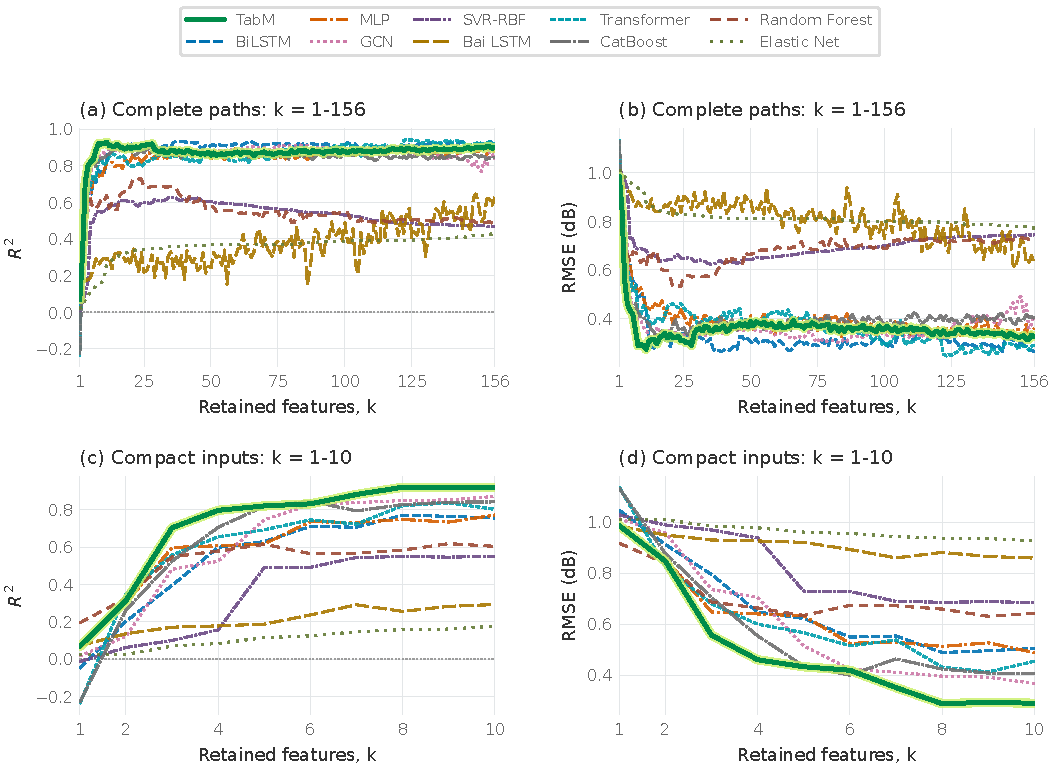
\includegraphics[width=\textwidth]{Fig06_Ten_Model_RFE.pdf}
\caption{Local-test performance of ten models along their independent 156-to-1 RFE paths. The upper panels show the full range of retained dimensions, and the lower panels enlarge $k=1$--$10$. All states are evaluated on the same 687 test hours. Feature elimination proceeds from right to left.}
\label{fig:ten_model_rfe}
\end{figure*}

% Table 4: signed RMSE reductions and absolute R-squared differences.
% Generated by build_tables.py; source files: frozen_exports/local_metrics.csv
\begingroup
\begin{table*}[!htbp]
\centering
\caption{Local test comparison with TabM at representative retained feature counts. Upper panel: RMSE reduction (\%); lower panel: absolute $R^2$ difference.}\label{tab:Table04_Local_Ten_Model_Comparison}
\small\setlength{\tabcolsep}{4pt}\renewcommand{\arraystretch}{1.12}
\resizebox{\textwidth}{!}{%
\begin{tabular}{lrrrrrrrrrrr}
\toprule
Weather & $k$ & TabM RMSE & BiLSTM & MLP & GCN & SVR & Bai & Transf. & CB & RF & EN \\
\midrule
Overall & 156 & 0.3250 & -22.80 & +9.65 & +21.68 & +56.33 & +47.88 & -12.36 & +18.70 & +55.55 & +57.94 \\
Overall & 10 & 0.2891 & +42.66 & +40.74 & +21.07 & +57.75 & +66.35 & +36.30 & +28.66 & +55.01 & +68.82 \\
Overall & 5 & 0.4324 & +30.47 & +31.59 & +15.90 & +40.67 & +53.03 & +23.58 & +0.53 & +31.74 & +55.00 \\
Overall & 1 & 0.9858 & +5.82 & +0.37 & +2.65 & +4.13 & -0.20 & +13.29 & +12.97 & -7.50 & +2.33 \\
Rain & 156 & 0.4398 & -16.94 & +17.34 & +10.23 & +47.37 & +43.43 & -33.43 & +14.43 & +25.41 & +55.14 \\
Rain & 10 & 0.4708 & +48.85 & -16.83 & +13.80 & +45.43 & +56.75 & +43.10 & +23.86 & +31.18 & +57.88 \\
Rain & 5 & 0.5449 & +49.63 & +42.10 & +21.40 & +49.68 & +54.43 & +52.23 & +27.94 & +38.84 & +54.73 \\
Rain & 1 & 1.2882 & +3.56 & -6.26 & +1.41 & +5.09 & -1.36 & +6.87 & +5.28 & +2.80 & -6.08 \\
Overcast & 156 & 0.5158 & -29.49 & -8.53 & -5.90 & +26.80 & +20.63 & -25.41 & -12.13 & +6.91 & +34.61 \\
Overcast & 10 & 0.3153 & -15.18 & +35.41 & +7.53 & +54.39 & +61.98 & +3.16 & +14.99 & +37.00 & +65.56 \\
Overcast & 5 & 0.5292 & -5.51 & -27.91 & -28.01 & +32.68 & +41.07 & -31.64 & -34.30 & +3.14 & +44.27 \\
Overcast & 1 & 0.9352 & +4.79 & +0.23 & +5.81 & +6.55 & +0.86 & +14.05 & +29.42 & -11.19 & +4.71 \\
Clear/dry & 156 & 0.1242 & +13.70 & +37.88 & +47.13 & +62.59 & +59.27 & +33.92 & +41.51 & +59.05 & +69.16 \\
Clear/dry & 10 & 0.2117 & +42.28 & +43.42 & +18.04 & +28.13 & +48.25 & +27.36 & +17.32 & +19.08 & +56.47 \\
Clear/dry & 5 & 0.2682 & +48.87 & +33.75 & -1.99 & +22.07 & +42.86 & +28.02 & +22.73 & +16.41 & +49.88 \\
Clear/dry & 1 & 0.5469 & +15.67 & +8.26 & +7.56 & +1.16 & -1.32 & +31.94 & +18.00 & -2.20 & +5.89 \\
Other & 156 & 0.3172 & -30.85 & +22.15 & +44.43 & +73.94 & +66.48 & -6.51 & +43.04 & +75.96 & +72.70 \\
Other & 10 & 0.3199 & +54.23 & +53.07 & +34.39 & +70.23 & +76.29 & +49.45 & +43.75 & +71.62 & +77.60 \\
Other & 5 & 0.5423 & +23.13 & +44.58 & +34.76 & +47.94 & +61.59 & +25.81 & -10.88 & +45.58 & +62.46 \\
Other & 1 & 1.4948 & +3.44 & -0.59 & +0.07 & +3.67 & -0.04 & +6.13 & +2.50 & -10.75 & +2.12 \\
\bottomrule
\end{tabular}
}
\par\smallskip\textbf{(b) Absolute $R^2$ difference}\par\smallskip
\resizebox{\textwidth}{!}{%
\begin{tabular}{lrrrrrrrrrrr}
\toprule
Weather & $k$ & TabM $R^2$ & BiLSTM & MLP & GCN & SVR & Bai & Transf. & CB & RF & EN \\
\midrule
Overall & 156 & 0.8988 & -0.0341 & +0.0228 & +0.0638 & +0.4297 & +0.2714 & -0.0211 & +0.0519 & +0.4111 & +0.4710 \\
Overall & 10 & 0.9199 & +0.1635 & +0.1480 & +0.0485 & +0.3685 & +0.6272 & +0.1173 & +0.0773 & +0.3156 & +0.7435 \\
Overall & 5 & 0.8208 & +0.1915 & +0.2036 & +0.0742 & +0.3298 & +0.6330 & +0.1277 & +0.0019 & +0.2054 & +0.7054 \\
Overall & 1 & 0.0686 & +0.1186 & +0.0070 & +0.0515 & +0.0819 & -0.0037 & +0.3075 & +0.2984 & -0.1255 & +0.0450 \\
Rain & 156 & 0.8855 & -0.0308 & +0.0531 & +0.0276 & +0.2988 & +0.2433 & -0.0502 & +0.0419 & +0.0913 & +0.4544 \\
Rain & 10 & 0.8688 & +0.3702 & -0.0351 & +0.0454 & +0.3093 & +0.5700 & +0.2739 & +0.0951 & +0.1457 & +0.6082 \\
Rain & 5 & 0.8243 & +0.5167 & +0.3484 & +0.1087 & +0.5181 & +0.6702 & +0.5941 & +0.1627 & +0.2940 & +0.6815 \\
Rain & 1 & 0.0180 & +0.0739 & -0.1122 & +0.0283 & +0.1082 & -0.0262 & +0.1503 & +0.1126 & +0.0575 & -0.1094 \\
Overcast & 156 & 0.7243 & -0.1113 & -0.0416 & -0.0299 & +0.2388 & +0.1620 & -0.1004 & -0.0564 & +0.0424 & +0.3691 \\
Overcast & 10 & 0.8970 & -0.0254 & +0.1439 & +0.0175 & +0.3923 & +0.6100 & +0.0068 & +0.0395 & +0.1566 & +0.7656 \\
Overcast & 5 & 0.7098 & -0.0295 & -0.1128 & -0.1131 & +0.3501 & +0.5455 & -0.1227 & -0.1293 & +0.0191 & +0.6441 \\
Overcast & 1 & 0.0937 & +0.0935 & +0.0042 & +0.1153 & +0.1316 & +0.0158 & +0.3204 & +0.9129 & -0.1733 & +0.0918 \\
Clear/dry & 156 & 0.9520 & +0.0164 & +0.0764 & +0.1236 & +0.2948 & +0.2411 & +0.0619 & +0.0923 & +0.2381 & +0.4565 \\
Clear/dry & 10 & 0.8606 & +0.2790 & +0.2960 & +0.0681 & +0.1305 & +0.3811 & +0.1248 & +0.0645 & +0.0735 & +0.5964 \\
Clear/dry & 5 & 0.7763 & +0.6321 & +0.2861 & -0.0087 & +0.1446 & +0.4615 & +0.2081 & +0.1510 & +0.0965 & +0.6667 \\
Clear/dry & 1 & 0.0699 & +0.3778 & +0.1749 & +0.1584 & +0.0219 & -0.0241 & +1.0781 & +0.4533 & -0.0396 & +0.1200 \\
Other & 156 & 0.9562 & -0.0182 & +0.0285 & +0.0980 & +0.6005 & +0.3457 & -0.0052 & +0.0911 & +0.7133 & +0.5437 \\
Other & 10 & 0.9555 & +0.1680 & +0.1577 & +0.0589 & +0.4580 & +0.7476 & +0.1297 & +0.0962 & +0.5082 & +0.8426 \\
Other & 5 & 0.8720 & +0.0886 & +0.2887 & +0.1727 & +0.3441 & +0.7394 & +0.1045 & -0.0239 & +0.3041 & +0.7802 \\
Other & 1 & 0.0278 & +0.0705 & -0.0114 & +0.0013 & +0.0754 & -0.0008 & +0.1311 & +0.0504 & -0.1796 & +0.0425 \\
\bottomrule
\end{tabular}
}
\par\smallskip
\begin{minipage}{\textwidth}\footnotesize Positive values favor TabM; negative values favor the column model. Panel (a): $100(\mathrm{RMSE}_{baseline}-\mathrm{RMSE}_{TabM})/\mathrm{RMSE}_{baseline}$. Panel (b): $\Delta R^2=R^2_{TabM}-R^2_{baseline}$ (absolute difference, not a percentage). Absolute TabM values are included. Test counts: overall 687, rain 51, overcast 158, clear/dry 322, other 156. SVR=SVR-RBF; Bai=Bai LSTM; Transf.=Transformer; CB=CatBoost; RF=Random Forest; EN=Elastic Net. All 156 states remain in the accompanying numeric export.\end{minipage}
\end{table*}
\endgroup


At the common ten-feature state, TabM achieves the lowest overall RMSE among the ten models: 0.2891~dB, with $R^2=0.9199$. GCN and CatBoost obtain RMSEs of 0.3663 and 0.4052~dB, respectively, corresponding to reductions of 21.07\% and 28.66\% with TabM. Across all nine comparators, the overall RMSE reduction ranges from 21.07\% to 68.82\%.

For TabM itself, reducing the input from 156 to ten features lowers overall test RMSE from 0.3250 to 0.2891~dB and raises $R^2$ from 0.8988 to 0.9199. This state uses 93.59\% fewer inputs and has an 11.05\% lower overall RMSE. The main weather-specific improvement occurs under dry-overcast conditions, where RMSE decreases from 0.5158 to 0.3153~dB. Rainy-hour RMSE changes from 0.4398 to 0.4708~dB.

The model ordering also depends on weather: at $k=10$, MLP has a lower rainy-hour RMSE than TabM, while BiLSTM has a lower dry-overcast RMSE. Thus, TabM's leading result concerns the overall error at the common compact-input state. The complete paths show that model ranking and the effect of further elimination vary with the retained feature set.

\subsubsection{Equal-dimensional comparison of the two TabM paths}

The role of vertically resolved inputs is examined by comparing the independently constructed 156-candidate and 50-candidate TabM paths at the same retained dimension. Figure~\ref{fig:tabm_two_pools} covers $k=1$--$50$, with an enlargement of $k=1$--$10$. The full-pool path may retain both base and pressure-level variables; the base-pool path is restricted to the 50 non-vertically-resolved candidates. Table~\ref{tab:Table05_TabM_Independent_Pool_Comparison} reports absolute metrics for both paths.

% Figure 7: equal-k comparison of independent starting pools.
\begin{figure*}[t]
\centering
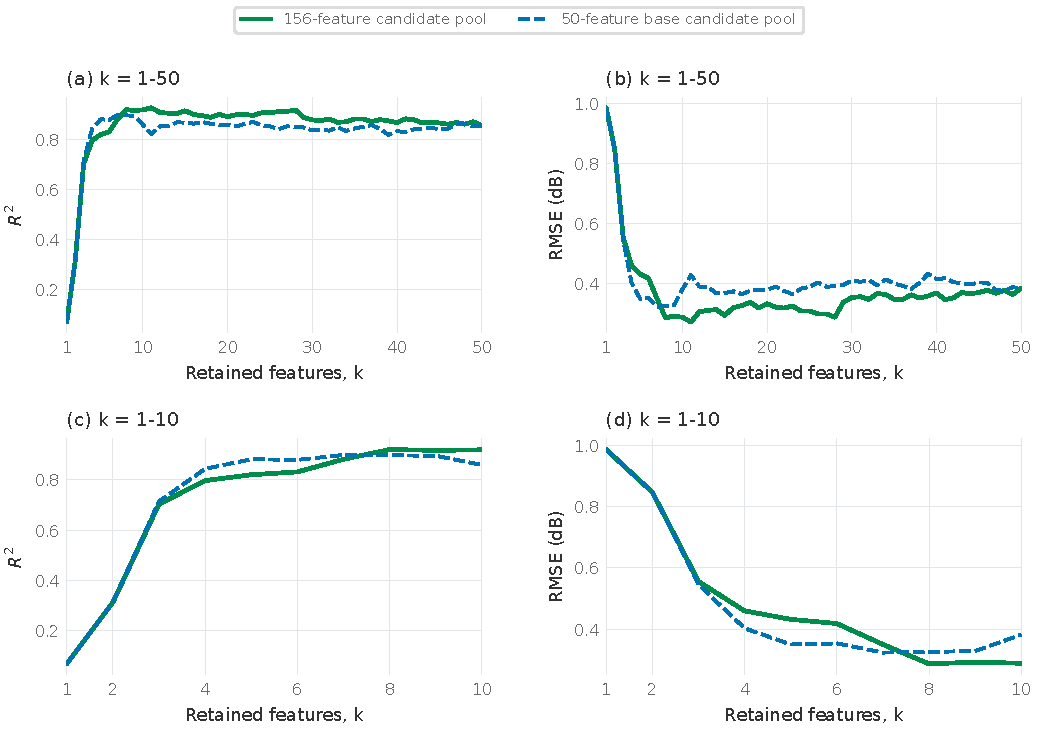
\includegraphics[width=\textwidth]{Fig07_TabM_Independent_RFE_Paths.pdf}
\caption{TabM comparison at equal retained dimensions for two independent RFE paths starting from 156 full-pool features and 50 non-vertically-resolved base features. Upper panels compare $k=1$--$50$; lower panels enlarge $k=1$--$10$. Both paths use the same network settings and 687 local test hours.}
\label{fig:tabm_two_pools}
\end{figure*}

% Table 5: pool subscripts indicate the initial candidate pool.
% Generated by build_tables.py; source files: frozen_exports/tabm_same_k.csv
\begingroup
\begin{table*}[!htbp]
\centering
\caption{TabM on two independently eliminated candidate pools at equal $k$ (local test).}\label{tab:Table05_TabM_Independent_Pool_Comparison}
\small\setlength{\tabcolsep}{4pt}\renewcommand{\arraystretch}{1.12}
\resizebox{\textwidth}{!}{%
\begin{tabular}{lrrrrrrr}
\toprule
Weather & $k$ & RMSE$_{156}$ & RMSE$_{50}$ & RMSE$_{50}-\mathrm{RMSE}_{156}$ & $R^2_{156}$ & $R^2_{50}$ & $R^2_{156}-R^2_{50}$ \\
\midrule
Overall & 50 & 0.3862 & 0.3843 & -0.0020 & 0.8570 & 0.8585 & -0.0014 \\
Overall & 25 & 0.3096 & 0.3902 & +0.0806 & 0.9081 & 0.8541 & +0.0541 \\
Overall & 10 & 0.2891 & 0.3823 & +0.0932 & 0.9199 & 0.8599 & +0.0600 \\
Overall & 5 & 0.4324 & 0.3503 & -0.0821 & 0.8208 & 0.8824 & -0.0616 \\
Overall & 1 & 0.9858 & 0.9858 & +0.0000 & 0.0686 & 0.0686 & +0.0000 \\
Rain & 50 & 0.4737 & 0.6018 & +0.1281 & 0.8672 & 0.7857 & +0.0815 \\
Rain & 25 & 0.3659 & 0.5714 & +0.2055 & 0.9208 & 0.8068 & +0.1140 \\
Rain & 10 & 0.4708 & 0.4350 & -0.0359 & 0.8688 & 0.8881 & -0.0192 \\
Rain & 5 & 0.5449 & 0.5973 & +0.0524 & 0.8243 & 0.7889 & +0.0354 \\
Rain & 1 & 1.2882 & 1.2882 & +0.0000 & 0.0180 & 0.0180 & +0.0000 \\
Overcast & 50 & 0.6103 & 0.5818 & -0.0285 & 0.6140 & 0.6492 & -0.0352 \\
Overcast & 25 & 0.4412 & 0.5722 & +0.1310 & 0.7983 & 0.6608 & +0.1375 \\
Overcast & 10 & 0.3153 & 0.5500 & +0.2347 & 0.8970 & 0.6865 & +0.2105 \\
Overcast & 5 & 0.5292 & 0.3218 & -0.2074 & 0.7098 & 0.8927 & -0.1829 \\
Overcast & 1 & 0.9352 & 0.9352 & +0.0000 & 0.0937 & 0.0937 & +0.0000 \\
Clear/dry & 50 & 0.1353 & 0.1477 & +0.0124 & 0.9431 & 0.9322 & +0.0109 \\
Clear/dry & 25 & 0.1259 & 0.1491 & +0.0232 & 0.9507 & 0.9309 & +0.0198 \\
Clear/dry & 10 & 0.2117 & 0.2300 & +0.0183 & 0.8606 & 0.8355 & +0.0252 \\
Clear/dry & 5 & 0.2682 & 0.2857 & +0.0175 & 0.7763 & 0.7461 & +0.0302 \\
Clear/dry & 1 & 0.5469 & 0.5469 & +0.0000 & 0.0699 & 0.0699 & +0.0000 \\
Other & 50 & 0.4104 & 0.3795 & -0.0310 & 0.9267 & 0.9373 & -0.0106 \\
Other & 25 & 0.3854 & 0.4317 & +0.0463 & 0.9354 & 0.9189 & +0.0165 \\
Other & 10 & 0.3199 & 0.4076 & +0.0877 & 0.9555 & 0.9277 & +0.0278 \\
Other & 5 & 0.5423 & 0.3878 & -0.1545 & 0.8720 & 0.9346 & -0.0625 \\
Other & 1 & 1.4948 & 1.4948 & +0.0000 & 0.0278 & 0.0278 & +0.0000 \\
\bottomrule
\end{tabular}
}
\par\smallskip
\begin{minipage}{\textwidth}\footnotesize Subscripts denote the starting candidate pool, not the number of inputs at the evaluated state. RMSE is in dB. The 50-feature pool contains surface, single-level diagnostic and column-integrated variables. Positive difference columns favor the 156-pool path; negative differences are retained. Table~S1 lists both retained sets at $k=10$. The full $k=1$--50 export is included.\end{minipage}
\end{table*}
\endgroup


At $k=10$, the full-pool path obtains an overall RMSE of 0.2891~dB, compared with 0.3823~dB for the base-pool path, a reduction of 24.38\%. The corresponding $R^2$ values are 0.9199 and 0.8599. Under dry-overcast conditions, RMSE decreases from 0.5500 to 0.3153~dB, a reduction of 42.67\%. Clear-dry and other-weather RMSEs also decrease, whereas the base-pool path has the lower rainy-hour RMSE at this dimension.

The comparison depends on the retained dimension. At $k=25$, the full-pool path has the lower overall RMSE, while at $k=5$ the base-pool path is better, with RMSEs of 0.3503 and 0.4324~dB, respectively. These results locate the benefit of access to vertical information within the interaction between candidate composition and input dimension. At the common ten-feature state, pressure-level candidates enable a more accurate compact local estimator with the network and training settings held fixed.

The exact ten-feature sets are listed in Table~\ref{tab:TableS01_TabM_K10_Retained_Features}. Five features are shared: convective available potential energy, maximum 2-m temperature since the previous post-processing time, K index, vertically integrated eastward water-vapour flux, and total-column ozone. The full-pool path additionally retains ozone mass mixing ratio at 850~hPa, specific humidity at 650~hPa, temperature at 300~hPa, and the eastward wind component at 5 and 1~hPa.

The other five base-pool features are surface pressure, mean large-scale precipitation rate, vertically integrated eastward mass flux, vertically integrated eastward ozone flux, and vertically integrated northward heat flux. The full-pool subset therefore combines stability and column descriptors with variables resolved at distinct atmospheric levels. These retained sets describe model-dependent predictive selections; their listed order is the input order and does not rank their individual importance.

\subsection{Frozen Evaluation at the UK Sites}
\label{subsec:uk_frozen_hourly}

External evaluation uses the local $k=10,\ldots,1$ checkpoints of each of the ten models, giving 100 frozen model states. Each state retains its local feature identities and order, preprocessing parameters, target transformation, and fitted model parameters. The UK data are passed through these fixed estimators without training, preprocessing refitting, or feature reselection. Accordingly, the horizontal axis in Fig.~\ref{fig:uk_frozen_models} indexes states along the local RFE paths.

The evaluation includes 5593 valid station-hours: 3382 at Chilbolton and 2211 at Sparsholt. Figure~\ref{fig:uk_frozen_models} reports pooled and station-specific performance. Table~\ref{tab:Table06_UK_Frozen_Model_Comparison} gives the pooled weather-specific comparisons at representative dimensions, while Table~\ref{tab:TableS02} provides the absolute $k=10$ metrics. In the hourly UK grouping, the other-weather category includes clear-dry hours.

% Figure 8: frozen inference, not an RFE procedure performed in the UK.
\begin{figure*}[t]
\centering
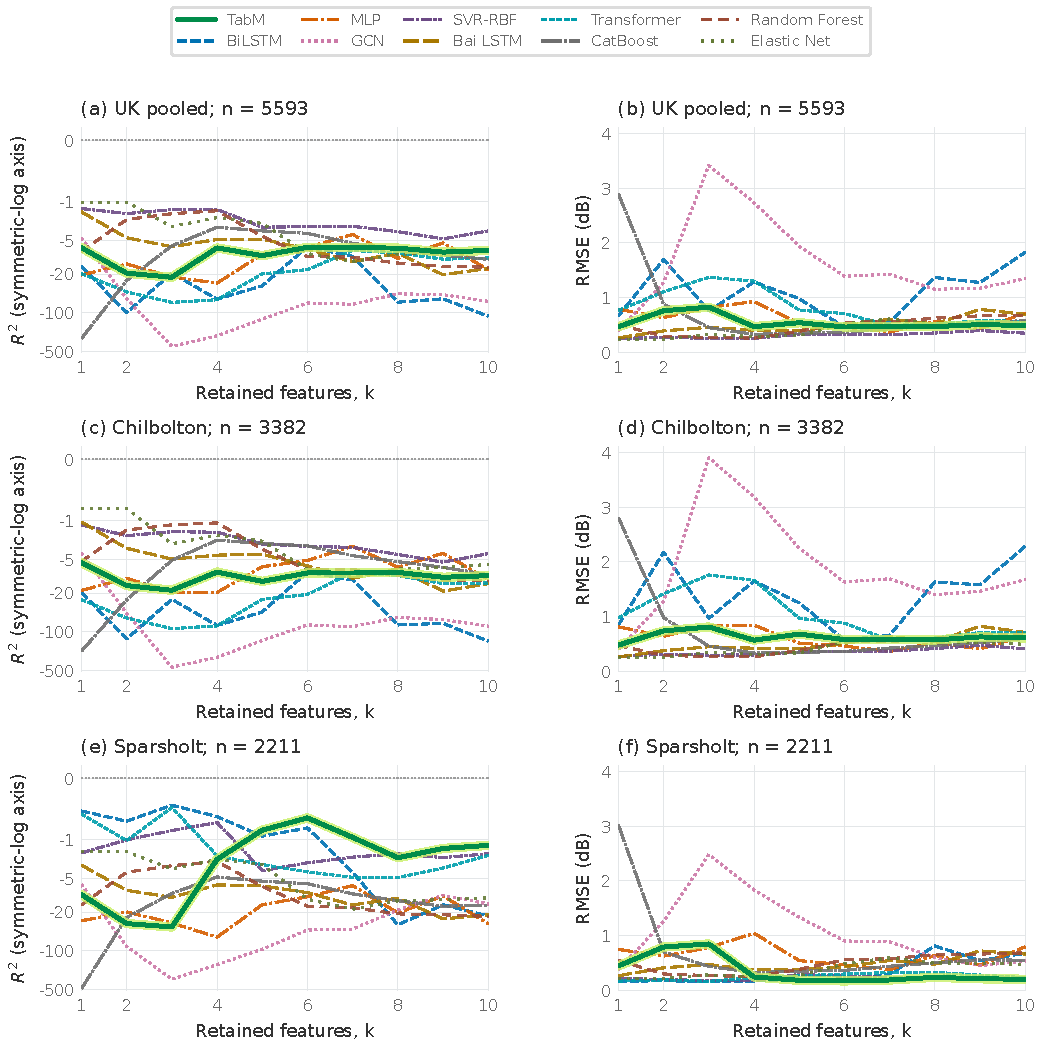
\includegraphics[width=\textwidth]{Fig08_UK_Frozen_Model_Comparison.pdf}
\caption{Evaluation of 100 frozen local model states at the UK sites, comprising ten models at $k=1$--$10$. Rows show the pooled sites, Chilbolton, and Sparsholt. The $R^2$ panels use explicitly labeled symmetric-log axes to retain the complete negative range; RMSE panels use linear axes.}
\label{fig:uk_frozen_models}
\end{figure*}

% Table 6: relative comparisons; absolute metrics are in Table S2.
% Generated by build_tables.py; source files: frozen_exports/uk_metrics.csv
\begingroup
\begin{table*}[!htbp]
\centering
\caption{Frozen UK pooled comparison with TabM. Upper panel: RMSE reduction (\%); lower panel: absolute $R^2$ difference.}\label{tab:Table06_UK_Frozen_Model_Comparison}
\small\setlength{\tabcolsep}{4pt}\renewcommand{\arraystretch}{1.12}
\resizebox{\textwidth}{!}{%
\begin{tabular}{lrrrrrrrrrrr}
\toprule
Weather & $k$ & TabM RMSE & BiLSTM & MLP & GCN & SVR & Bai & Transf. & CB & RF & EN \\
\midrule
Overall & 10 & 0.4946 & +72.95 & +31.10 & +63.30 & -40.11 & +28.93 & +12.98 & +15.25 & +27.08 & -0.60 \\
Overall & 5 & 0.5447 & +44.55 & -2.62 & +71.92 & -63.53 & -34.55 & +29.67 & -54.34 & -40.96 & -72.98 \\
Overall & 1 & 0.4708 & +29.67 & +40.47 & -18.90 & -82.37 & -75.01 & +38.87 & +83.73 & +6.74 & -95.55 \\
Rain & 10 & 0.5802 & +59.90 & +52.73 & +55.26 & -32.16 & +23.03 & -39.28 & +17.23 & +25.80 & -10.11 \\
Rain & 5 & 0.6520 & -7.02 & +12.52 & +53.09 & -56.55 & -32.56 & -59.06 & -33.69 & -47.99 & -55.51 \\
Rain & 1 & 0.4955 & +7.89 & +28.34 & -17.68 & -32.84 & -12.15 & +19.20 & +71.93 & +25.63 & -31.66 \\
Overcast & 10 & 0.5380 & +71.55 & +12.83 & +61.23 & -50.07 & +30.55 & +18.89 & +11.70 & +36.56 & +1.15 \\
Overcast & 5 & 0.5076 & +49.51 & +12.11 & +74.97 & -46.42 & -16.54 & +42.00 & -46.05 & -28.62 & -54.54 \\
Overcast & 1 & 0.4826 & +29.36 & +42.11 & -26.23 & -91.01 & -109.30 & +39.40 & +84.08 & +0.63 & -122.22 \\
Other & 10 & 0.4208 & +77.49 & +28.99 & +68.24 & -32.22 & +29.31 & +17.42 & +18.85 & +0.75 & +1.25 \\
Other & 5 & 0.5432 & +48.09 & -37.89 & +72.75 & -86.95 & -58.31 & +28.25 & -76.06 & -50.39 & -106.79 \\
Other & 1 & 0.4523 & +34.53 & +41.84 & -12.86 & -105.89 & -93.96 & +42.50 & +85.05 & +3.05 & -116.53 \\
\bottomrule
\end{tabular}
}
\par\smallskip\textbf{(b) Absolute $R^2$ difference}\par\smallskip
\resizebox{\textwidth}{!}{%
\begin{tabular}{lrrrrrrrrrrr}
\toprule
Weather & $k$ & TabM $R^2$ & BiLSTM & MLP & GCN & SVR & Bai & Transf. & CB & RF & EN \\
\midrule
Overall & 10 & -7.5048 & +107.7556 & +9.4127 & +54.6465 & -4.1727 & +8.3351 & +2.7275 & +3.3365 & +7.4896 & -0.1008 \\
Overall & 5 & -9.3146 & +23.2334 & -0.5208 & +120.5109 & -6.4573 & -4.6169 & +10.5389 & -5.9844 & -5.1238 & -6.8674 \\
Overall & 1 & -6.7077 & +7.8758 & +14.0401 & -2.2558 & -5.3903 & -5.1911 & +12.9188 & +283.5476 & +1.1547 & -5.6921 \\
Rain & 10 & -1.3935 & +12.4916 & +8.3174 & +9.5639 & -1.0232 & +1.6468 & -1.1597 & +1.1003 & +1.9535 & -0.4194 \\
Rain & 5 & -2.0227 & -0.3835 & +0.9272 & +10.7159 & -1.7893 & -1.3026 & -1.8279 & -1.3316 & -1.6426 & -1.7727 \\
Rain & 1 & -0.7453 & +0.3119 & +1.6533 & -0.4851 & -0.7563 & -0.3576 & +0.9280 & +20.4128 & +1.4101 & -0.7385 \\
Overcast & 10 & -23.2894 & +275.7933 & +7.6749 & +137.3082 & -13.5044 & +26.0735 & +12.6324 & +6.8654 & +36.0700 & +0.5694 \\
Overcast & 5 & -20.6194 & +63.1760 & +6.3680 & +323.4097 & -11.5349 & -5.7009 & +42.6508 & -11.4839 & -8.5518 & -12.5670 \\
Overcast & 1 & -18.5460 & +19.6210 & +38.7745 & -7.2800 & -14.1887 & -15.0840 & +33.6812 & +752.0321 & +0.2467 & -15.5878 \\
Other & 10 & -32.9942 & +636.6440 & +33.4224 & +302.9786 & -14.5478 & +34.0420 & +15.8514 & +17.6326 & +0.5190 & +0.8626 \\
Other & 5 & -55.6439 & +153.5539 & -26.8536 & +706.1933 & -40.4362 & -34.0424 & +53.3797 & -38.3704 & -31.6003 & -43.3970 \\
Other & 1 & -38.2645 & +52.3465 & +76.8271 & -8.4398 & -30.0021 & -28.8274 & +79.4898 & +1717.6671 & +2.5055 & -30.8901 \\
\bottomrule
\end{tabular}
}
\par\smallskip
\begin{minipage}{\textwidth}\footnotesize Positive values favor TabM; negative values favor the column model. Panel (a): $100(\mathrm{RMSE}_{baseline}-\mathrm{RMSE}_{TabM})/\mathrm{RMSE}_{baseline}$. Panel (b): $\Delta R^2=R^2_{TabM}-R^2_{baseline}$ (absolute difference, not a percentage). Absolute TabM values are included.  UK counts: overall 5593, rain 735, overcast 2317, other 2541. Other includes clear/dry hours in the frozen hourly UK evaluation. No local model is retrained on UK data. Station-specific absolute metrics are in Table~S2. Abbreviations follow Table~4.\end{minipage}
\end{table*}
\endgroup


At $k=10$, TabM obtains a pooled RMSE of 0.4946~dB, below seven of the nine comparators. Its RMSE is 12.98\% lower than that of Transformer and 15.25\% lower than that of CatBoost. SVR-RBF and Elastic Net obtain lower pooled RMSEs of 0.3530 and 0.4916~dB, respectively. TabM's station-specific RMSE is 0.6136~dB at Chilbolton and 0.2070~dB at Sparsholt.

The absolute metrics provide a different perspective from these relative rankings. At $k=10$, all ten models have negative pooled $R^2$ values; TabM obtains $R^2=-7.5048$. Its squared prediction error therefore exceeds the squared variation around the UK cohort's observed mean. The locally observed compact-input advantage consequently does not establish accurate frozen transfer across these sites. The UK results characterize the dependence of transfer performance on the model, retained feature set, and evaluation site, and provide the hourly baseline for the second-scale combination examined in Section~IV.

